\documentclass[tikz,border=6pt]{standalone}
\usetikzlibrary{decorations.markings,arrows.meta}

\begin{document}
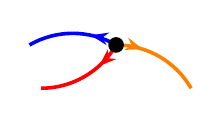
\begin{tikzpicture}[
    % 定义带箭头的 loop 样式
    loopStyle/.style={
        line width=1.3pt,
        postaction={decorate},
        decoration={markings, mark=at position 0.30 with {\arrow{Stealth[length=2.2mm,width=1.6mm]}}}
    }
]
    % 核心原理：左弧线从原点荡上去，右弧线再荡回原点，形成完美闭合的叶片
    % Top Petal (朝上)
    \draw[loopStyle, draw=blue] (0,0) 
        arc[start angle=60, end angle=120, radius=1.1];
     
                      
    % Left Petal (旋转 120 度)
    \draw[loopStyle, draw=red, rotate=120] (0,0) 
        arc[start angle=210, end angle=150, radius=1.1];
        
                                                
    % Right Petal (旋转 -120 度)
    \draw[loopStyle, draw=orange, rotate=-120] (0,0) 
        arc[start angle=210, end angle=150, radius=1.1];
       

    % 原点处的顶点
    \node[circle, fill=black, inner sep=2pt] at (0,0) {};
\end{tikzpicture}
\end{document}